\chapter{Введение}
Целью данной лабораторной работы является изучение архитектуры гетерогенных вычислительных систем и технологии разработки ускорителей вычислений на базе ПЛИС фирмы Xilinx.

Для достижения данной цели необходимо выполнить следующие задачи:
\begin{enumerate}
	\item Изучить основные сведения о платформе Xilinx Alveo U200;
	\item Разработать RTL описание ускорителя вычислений по индивидуальному варианту;
	\item Выполнить генерацию ядра ускорителя;
	\item Выполнить синтез и сборку бинарного модуля ускорителя;
	\item Разработать и отладить тестирующее ПО на серверной хост-платформе;
	\item Провести тесты работы ускорителя вычислений.
\end{enumerate}

\chapter{Функциональная схема разрабатываемой аппаратной системы}
\begin{figure}[ph!]
	\center{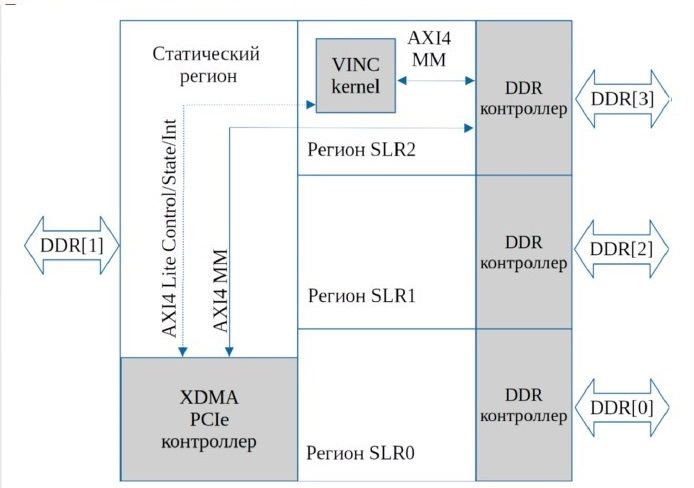
\includegraphics[scale=0.7]{func}}
	\caption{Функциональная схема разрабатываемой аппаратной системы}
\end{figure}

\chapter{Изучение работы шины AXI}

В данном разделе приведены диаграммы, иллюстрирующие процесс рукопожатия и пакетного чтения.

\begin{figure}[ph!]
	\center{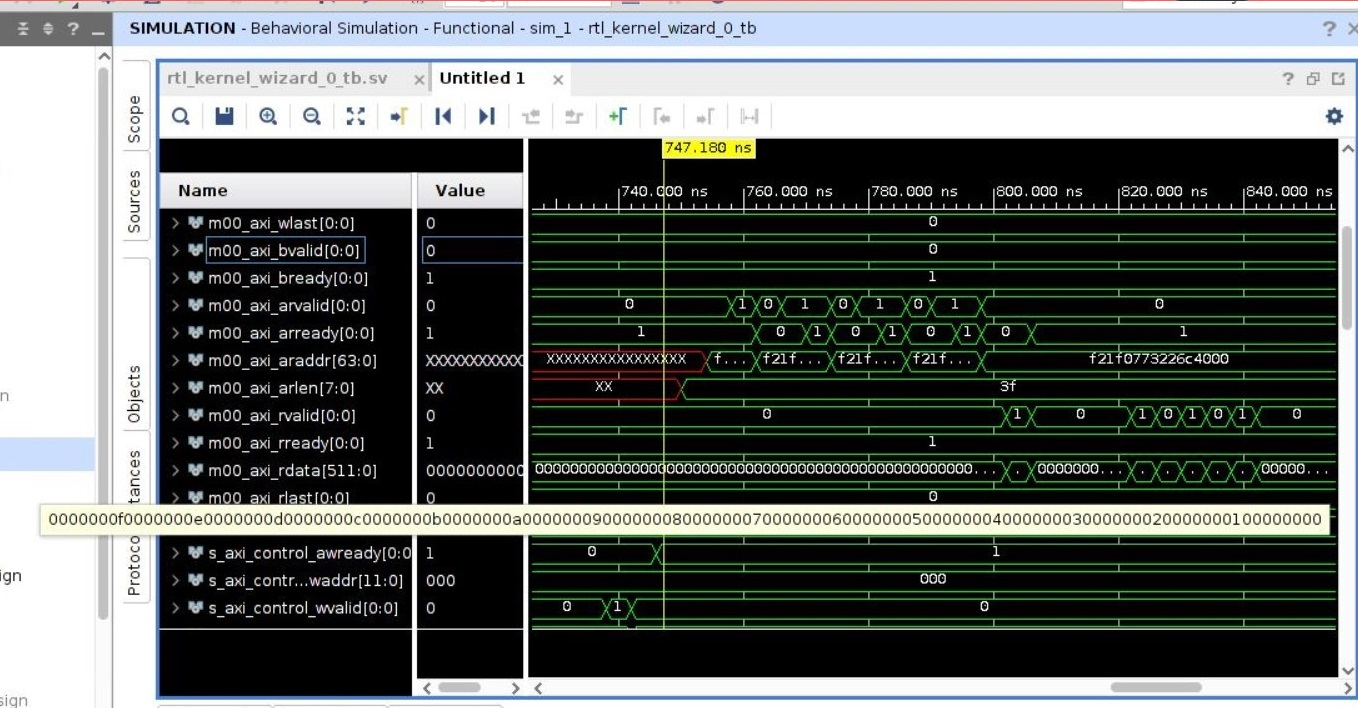
\includegraphics[scale=0.5]{reading}}
	\caption{Транзакция чтения данных вектора на шине AXI4 MM из DDR памяти}
\end{figure}

\begin{figure}[ph!]
	\center{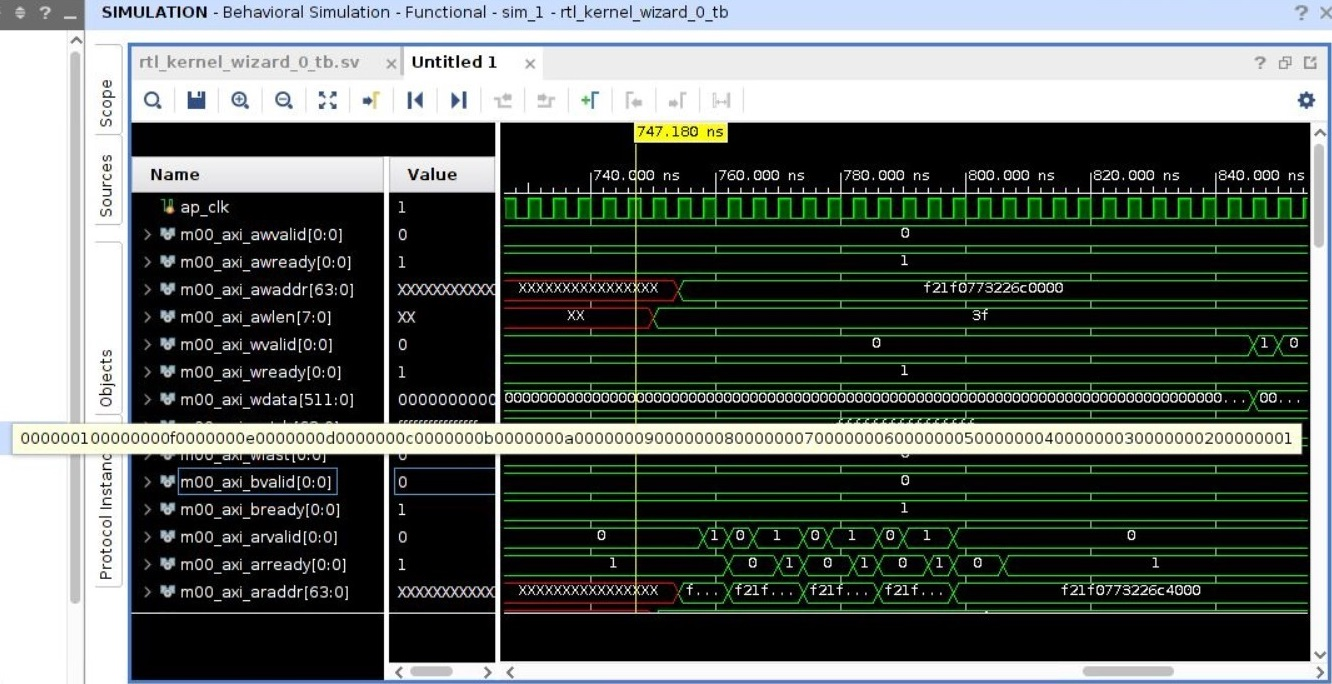
\includegraphics[scale=0.5]{writing}}
	\caption{Транзакция записи результата инкремента данных на шине AXI4 MM}
\end{figure}

\newpage

\begin{figure}[ph!]
	\center{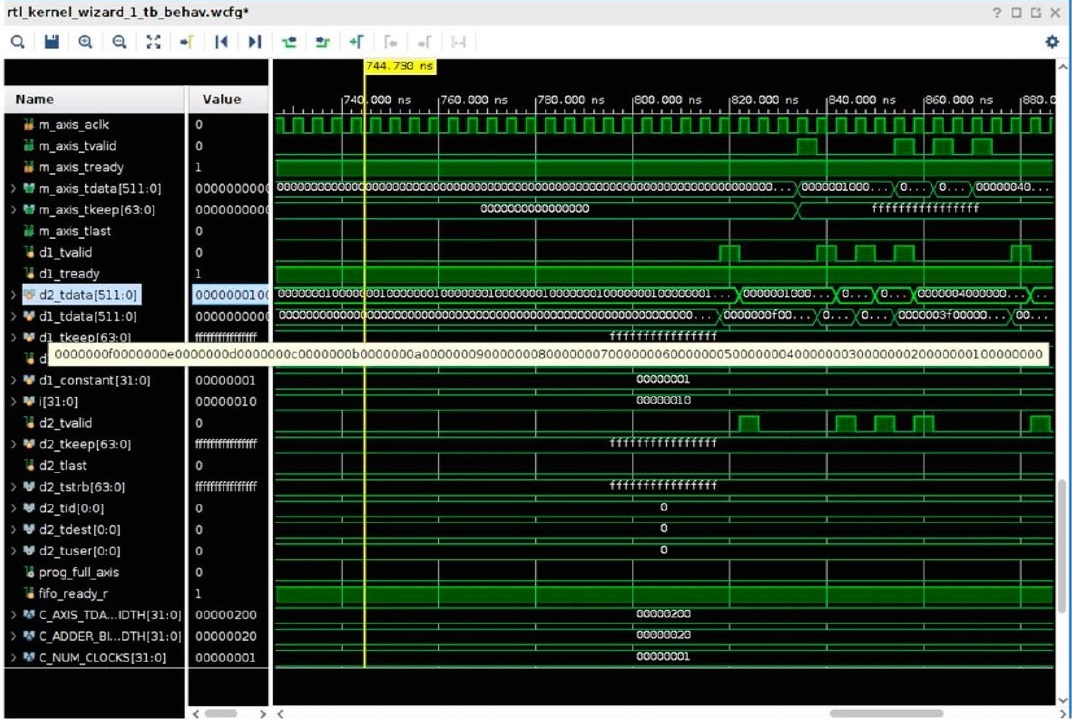
\includegraphics[scale=0.6]{inc}}
	\caption{Инкремент данных}
\end{figure}

Теперь изменим модуль rtl\_kernel\_wizard\_0\_example\_adder.v, чтобы ускоритель выполнял предложенную функцию:

R[i] = A[i]*16 + (10<<7)

Регион:

SLR1,DDR[1]

Фрагмент листинга кода функции аддера:

\begin{figure}[ph!]
	\center{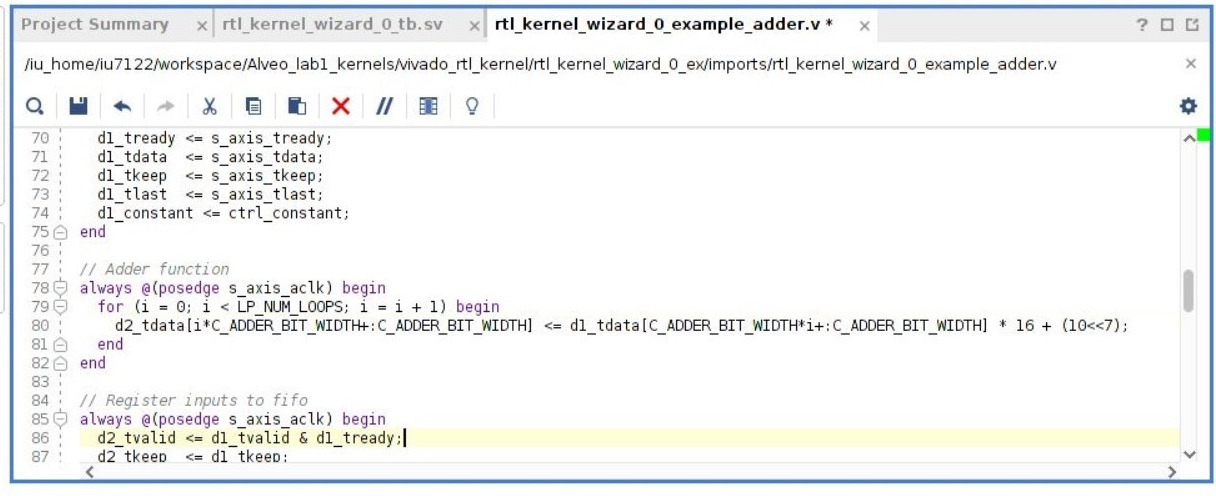
\includegraphics[scale=0.6]{adder_mod}}
	\caption{Фрагмент кода функции аддера}
\end{figure}


\begin{figure}[ph!]
	\center{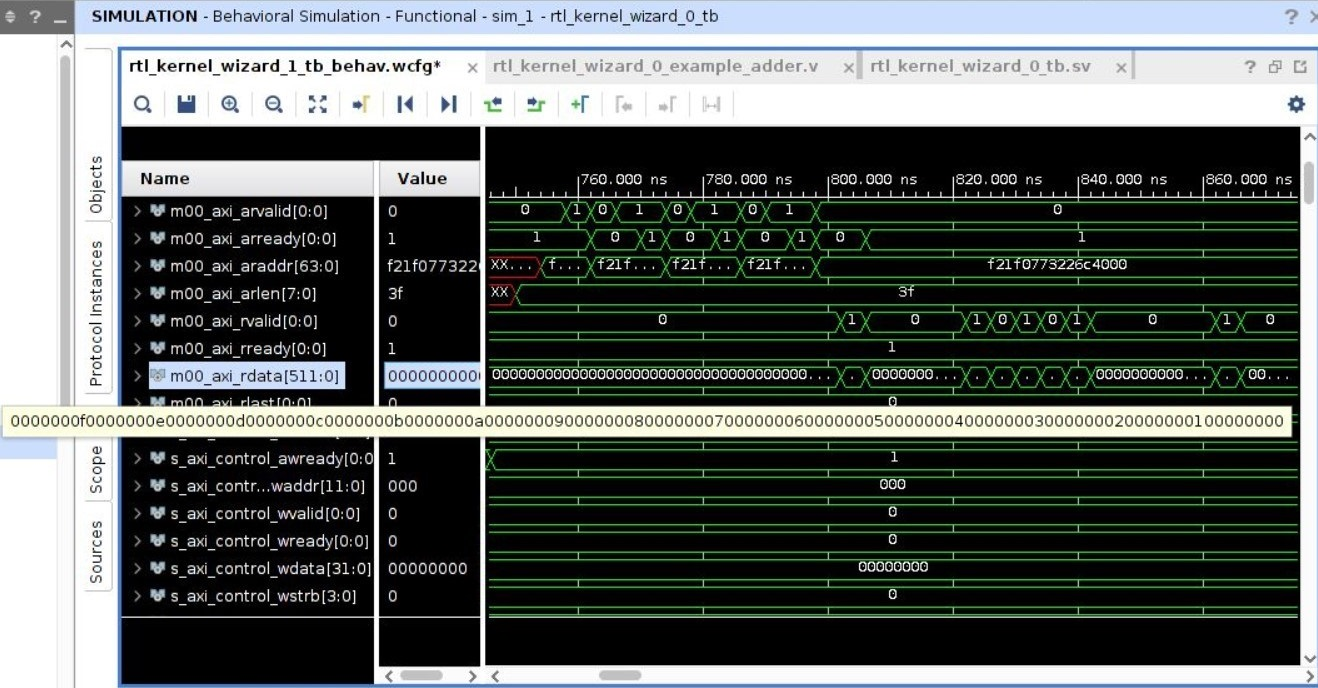
\includegraphics[scale=0.5]{reading_mod}}
	\caption{Транзакция чтения данных вектора на шине AXI4 MM из DDR памяти}
\end{figure}

\begin{figure}[ph!]
	\center{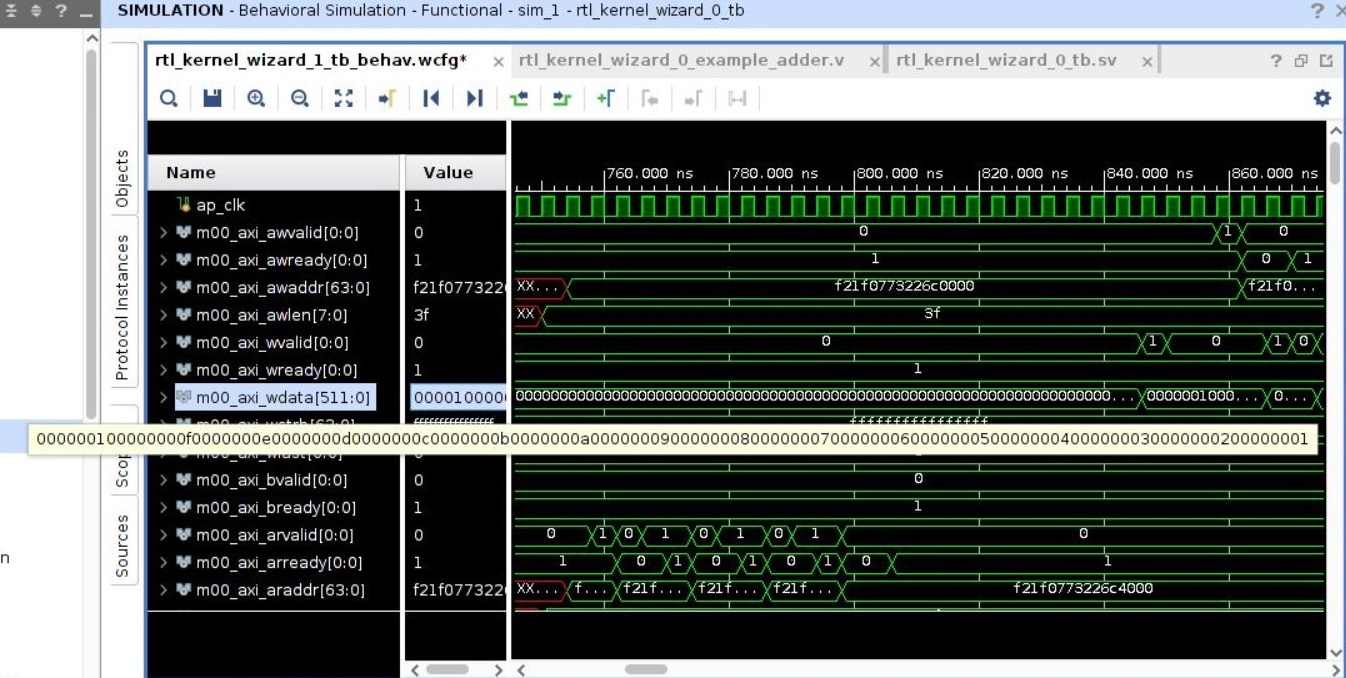
\includegraphics[scale=0.5]{writing_mod}}
	\caption{Транзакция записи результата инкремента данных на шине AXI4 MM}
\end{figure}

\newpage

\begin{figure}[ph!]
	\center{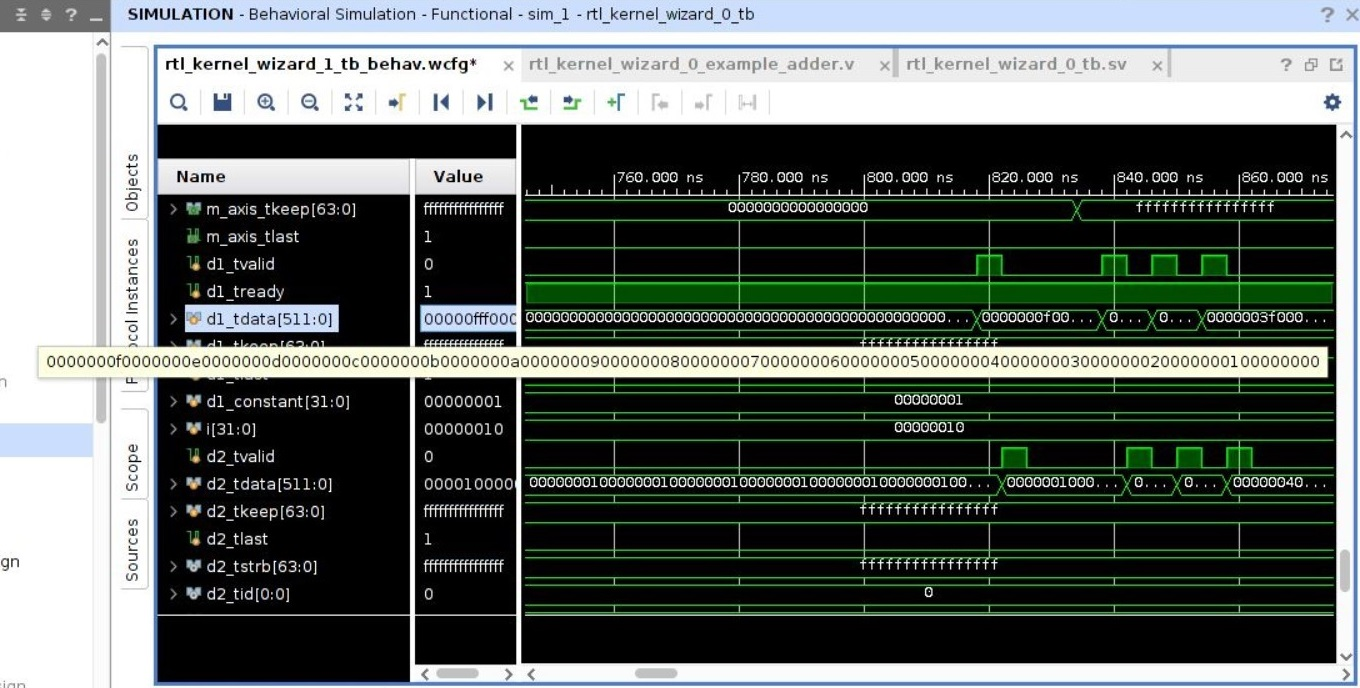
\includegraphics[scale=0.6]{inc_mod}}
	\caption{Инкремент данных}
\end{figure}

\chapter{Сборка проекта}

Для сборки проекта необходимо создать конфигурационного файла. В соответствии с вариантом требовалось использовать регионы памяти SL1, DDR[1]. Листинг файла конфигурации приведён ниже:

\begin{figure}[ph!]
	\center{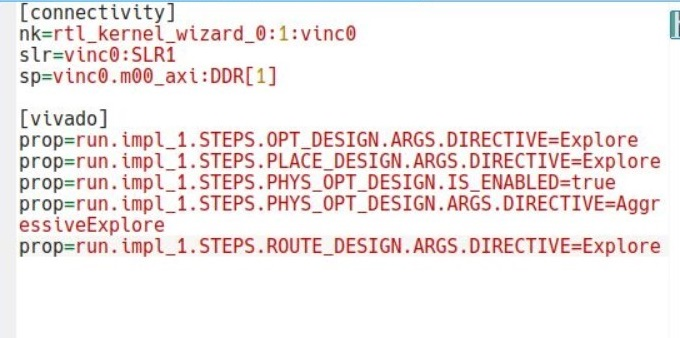
\includegraphics[scale=0.8]{config}}
	\caption{Инкремент данных}
\end{figure}

Листинг содержимого файла xclbin.info:
\begin{lstlisting}[label=some-code-1,caption=Содержимое файла xclbin.info]
==============================================================================
XRT Build Version: 2.8.743 (2020.2)
       Build Date: 2020-11-16 00:19:11
          Hash ID: 77d5484b5c4daa691a7f78235053fb036829b1e9
==============================================================================
xclbin Information
------------------
   Generated by:           v++ (2020.2) on 2020-11-18-05:13:29
   Version:                2.8.743
   Kernels:                rtl_kernel_wizard_0
   Signature:              
   Content:                Bitstream
   UUID (xclbin):          7df3cc3e-52be-4675-84ae-559c42cf1893
   Sections:               DEBUG_IP_LAYOUT, BITSTREAM, MEM_TOPOLOGY, IP_LAYOUT, 
                           CONNECTIVITY, CLOCK_FREQ_TOPOLOGY, BUILD_METADATA, 
                           EMBEDDED_METADATA, SYSTEM_METADATA, 
                           GROUP_CONNECTIVITY, GROUP_TOPOLOGY
==============================================================================
Hardware Platform (Shell) Information
-------------------------------------
   Vendor:                 xilinx
   Board:                  u200
   Name:                   xdma
   Version:                201830.2
   Generated Version:      Vivado 2018.3 (SW Build: 2568420)
   Created:                Tue Jun 25 06:55:20 2019
   FPGA Device:            xcu200
   Board Vendor:           xilinx.com
   Board Name:             xilinx.com:au200:1.0
   Board Part:             xilinx.com:au200:part0:1.0
   Platform VBNV:          xilinx_u200_xdma_201830_2
   Static UUID:            c102e7af-b2b8-4381-992b-9a00cc3863eb
   Feature ROM TimeStamp:  1561465320

Clocks
------
   Name:      DATA_CLK
   Index:     0
   Type:      DATA
   Frequency: 300 MHz

   Name:      KERNEL_CLK
   Index:     1
   Type:      KERNEL
   Frequency: 500 MHz

Memory Configuration
--------------------
   Name:         bank0
   Index:        0
   Type:         MEM_DDR4
   Base Address: 0x4000000000
   Address Size: 0x400000000
   Bank Used:    No

   Name:         bank1
   Index:        1
   Type:         MEM_DDR4
   Base Address: 0x5000000000
   Address Size: 0x400000000
   Bank Used:    Yes

   Name:         bank2
   Index:        2
   Type:         MEM_DDR4
   Base Address: 0x6000000000
   Address Size: 0x400000000
   Bank Used:    No

   Name:         bank3
   Index:        3
   Type:         MEM_DDR4
   Base Address: 0x7000000000
   Address Size: 0x400000000
   Bank Used:    No

   Name:         PLRAM[0]
   Index:        4
   Type:         MEM_DRAM
   Base Address: 0x3000000000
   Address Size: 0x20000
   Bank Used:    No

   Name:         PLRAM[1]
   Index:        5
   Type:         MEM_DRAM
   Base Address: 0x3000200000
   Address Size: 0x20000
   Bank Used:    No

   Name:         PLRAM[2]
   Index:        6
   Type:         MEM_DRAM
   Base Address: 0x3000400000
   Address Size: 0x20000
   Bank Used:    No
==============================================================================
Kernel: rtl_kernel_wizard_0

Definition
----------
   Signature: rtl_kernel_wizard_0 (uint num, int* axi00_ptr0)

Ports
-----
   Port:          s_axi_control
   Mode:          slave
   Range (bytes): 0x1000
   Data Width:    32 bits
   Port Type:     addressable

   Port:          m00_axi
   Mode:          master
   Range (bytes): 0xFFFFFFFFFFFFFFFF
   Data Width:    512 bits
   Port Type:     addressable

--------------------------
Instance:        vinc0
   Base Address: 0x1800000

   Argument:          num
   Register Offset:   0x010
   Port:              s_axi_control
   Memory:            <not applicable>

   Argument:          axi00_ptr0
   Register Offset:   0x018
   Port:              m00_axi
   Memory:            bank1 (MEM_DDR4)
==============================================================================
Generated By
------------
   Command:       v++
   Version:       2020.2 - 2020-11-18-05:13:29 (SW BUILD: 0)
   Command Line:  v++ --config /iu_home/iu7122/workspace/Alveo_lab1_kernels/
src/vitis_rtl_kernel/rtl_kernel_wizard_0/myconfig.cfg --connectivity.nk 
rtl_kernel_wizard_0:1:vinc0 --connectivity.slr vinc0:SLR1 --connectivity.sp vinc0.m00_axi:DDR[1] --input_files 
/iu_home/iu7122/workspace/Alveo_lab1_kernels/src/
vitis_rtl_kernel/rtl_kernel_wizard_0/rtl_kernel_wizard_0.xo --link --optimize 0 --output /iu_home/iu7122/workspace
/Alveo_lab1_kernels/src/vitis_rtl_kernel/rtl_kernel_wizard_0/vinc.xclbin --platform xilinx_u200_xdma_201830_2 --report_level 0
 --target hw --vivado.prop run.impl_1.STEPS.OPT_DESIGN.ARGS.DIRECTIVE=Explore 
--vivado.prop run.impl_1.STEPS.PLACE_DESIGN.ARGS.DIRECTIVE=Explore 
--vivado.prop run.impl_1.STEPS.PHYS_OPT_DESIGN.IS_ENABLED=true --vivado.prop 
run.impl_1.STEPS.PHYS_OPT_DESIGN.ARGS.DIRECTIVE=AggressiveExplore --vivado.prop
 run.impl_1.STEPS.ROUTE_DESIGN.ARGS.DIRECTIVE=Explore 
   Options:       --config /iu_home/iu7122/workspace/Alveo_lab1_kernels/src/vitis_rtl_kernel/
rtl_kernel_wizard_0/myconfig.cfg
         --connectivity.nk rtl_kernel_wizard_0:1:vinc0
         --connectivity.slr vinc0:SLR1
         --connectivity.sp vinc0.m00_axi:DDR[1]
         --input_files /iu_home/iu7122/workspace/Alveo_lab1_kernels/src/vitis_rtl_kernel/
rtl_kernel_wizard_0/rtl_kernel_wizard_0.xo
        --link
        --optimize 0
        --output /iu_home/iu7122/workspace/Alveo_lab1_kernels/src/vitis_rtl_kernel/
rtl_kernel_wizard_0/vinc.xclbin
        --platform xilinx_u200_xdma_201830_2
        --report_level 0
        --target hw
        --vivado.prop run.impl_1.STEPS.OPT_DESIGN.ARGS.DIRECTIVE=Explore
        --vivado.prop run.impl_1.STEPS.PLACE_DESIGN.ARGS.DIRECTIVE=Explore
        --vivado.prop run.impl_1.STEPS.PHYS_OPT_DESIGN.IS_ENABLED=true
        --vivado.prop run.impl_1.STEPS.PHYS_OPT_DESIGN.ARGS.DIRECTIVE=AggressiveExplore
        --vivado.prop run.impl_1.STEPS.ROUTE_DESIGN.ARGS.DIRECTIVE=Explore 
==============================================================================
User Added Key Value Pairs
--------------------------
   <empty>
==============================================================================
\end{lstlisting}

Содержимое файла v++\_vinc.log:

\begin{lstlisting}[label=some-code-2,caption=Содержимое файла v++\_vinc.log]
INFO: [v++ 60-1306] Additional information associated with this v++ link can be found at:
	Reports: /iu_home/iu7122/_x/reports/link
	Log files: /iu_home/iu7122/_x/logs/link
INFO: [v++ 60-1548] Creating build summary session with primary output /iu_home/iu7122/
workspace/ Alveo_lab1_kernels/src/vitis_rtl_kernel/rtl_kernel_wizard_0/
vinc.xclbin.link_summary, at Thu Oct 14 16:21:38 2021
INFO: [v++ 60-1316] Initiating connection to rulecheck server, at Thu Oct 14 16:21:39 2021
INFO: [v++ 60-1315] Creating rulecheck session with output '/iu_home/iu7122/_x/reports/link
 /v++_link_vinc_guidance.html', at Thu Oct 14 16:22:03 2021
INFO: [v++ 60-895]   Target platform: /opt/xilinx/platforms/xilinx_u200_xdma_201830_2/
 xilinx_u200_xdma_201830_2.xpfm
INFO: [v++ 60-1578]   This platform contains Device Support Archive '/opt/xilinx/platforms/ 
xilinx_u200_xdma_201830_2/hw/xilinx_u200_xdma_201830_2.dsa'
INFO: [v++ 74-74] Compiler Version string: 2020.2
INFO: [v++ 60-1302] Platform 'xilinx_u200_xdma_201830_2.xpfm' has been explicitly enable d for this release.
INFO: [v++ 60-629] Linking for hardware target
INFO: [v++ 60-423]   Target device: xilinx_u200_xdma_201830_2
INFO: [v++ 60-1332] Run 'run_link' status: Not started
INFO: [v++ 60-1443] [16:23:22] Run run_link: Step system_link: Started
INFO: [v++ 60-1453] Command Line: system_link --xo /iu_home/iu7122/workspace/
Alveo_la b1_kernels/src/vitis_rtl_kernel/rtl_kernel_wizard_0/rtl_kernel_wizard_0.xo --config 
/iu_home/iu7122/_x/link/int/syslinkConfig.ini --xpfm /opt/xilinx /platforms/xilinx_u200_xdma_201830_2/
xilinx_u200_xdma_201830_2.xpfm --target hw --output_dir /iu_home/iu7122/_x/link/int --temp _dir /iu_home/iu7122/_x/link/sys_link
INFO: [v++ 60-1454] Run Directory: /iu_home/iu7122/_x/link/run_link 
INFO: [SYSTEM_LINK 60-1316] Initiating connection to rulecheck server, at Thu Oct 14 16:23:41 2021
INFO: [SYSTEM_LINK 82-70] Extracting xo v3 file /iu_home/iu7122/wo rkspace/Alveo_lab1_kernels/src
/vitis_rtl_kernel/rtl_kernel_wizard_0/rtl_kernel_wizard_0.xo
INFO: [SYSTEM_LINK 82-53] Creating IP database /iu_home/iu7122/_x /link/sys_link/_sysl/.cdb/
xd_ip_db.xml
INFO: [SYSTEM_LINK 82-38] [16:23:44] build_xd_ip_db started: /data/ Xilinx/Vitis/2020.2/bin/
build_xd_ip_db -ip_search 0  -sds-pf /iu_home/iu7122/_x/link/sys_link
/xilinx_u200_xdma_201830_2.hpfm -clkid 0 -ip /iu_home/iu7122 /_x/link/sys_link/iprepo/
mycompany_com_kernel_rtl_kernel_wizard_0_1_0,rtl_kernel_wizard_0 - o /iu_home/iu7122/
_x/link/sys_link/_sysl/.cdb/xd_ip_db.xml
INFO: [SYSTEM_LINK 82-37] [16:24:34] build_xd_ip_db finished successf ully
Time (s): cpu = 00:00:52 ; elapsed = 00:00:50 . Memory (MB): peak = 1 557.891 ; gain = 0.000 ; free physical = 58457 ; free virtual = 305555
INFO: [SYSTEM_LINK 82-51] Create system connectivity graph 
INFO: [SYSTEM_LINK 82-102] Applying explicit connections to t he system connectivity graph: /iu_home/iu7122/_x/link/sys_link/cfgraph/cfgen_cfgraph.xml
INFO: [SYSTEM_LINK 82-38] [16:24:35] cfgen started: /data/Xi linx/Vitis/2020.2/bin/cfgen  -nk rtl_kernel_wizard_0:1:vinc0 -slr vinc0:SLR1 -sp vinc0.m00_axi:DDR[1] -dmclkid 0 -r /iu_home/iu7122/_x/link/sys _link/_sysl/.cdb/xd_ip_db.xml -o /iu_home/iu7122/_x/link/sys_link/cfgraph/cfgen_cfgraph.xml
INFO: [CFGEN 83-0] Kernel Specs:  
INFO: [CFGEN 83-0]   kernel: rtl_ker nel_wizard_0, num: 1  {vinc0}
INFO: [CFGEN 83-0] Port Specs: 
INFO: [CFGEN 83-0]   kernel: vinc0, k_port: m00_axi, sptag: DDR[1]
INFO: [CFGEN 83-0] SLR Specs: 
INFO: [CFGEN 83-0]   instance: vinc0, SLR: SLR1
INFO: [CFGEN 83-2228] Creating mapping for argument vinc0.axi00_ptr0 to DDR[1] for directive vinc0.m00_axi:DDR[1]
INFO: [SYSTEM_LINK 82-37] [16:25:13] cfgen finished successfully
Time (s): cpu = 00:00:37 ; elapsed = 00:00:39 . Memory (MB): peak = 1557.891 ; gain = 0.000 ; free physical = 58374 ; free virtual = 305472
INFO: [SYSTEM_LINK 82-52] Create top-level block diagram
INFO: [SYSTEM_LINK 82-38] [16:25:13] cf2bd started: /data/Xilinx/Vitis/2020.2/bin/ cf2bd  --linux --trace_buffer 1024 --input_file /iu_home/iu7122/_x/link/sys_link/cfgraph/cfgen_cfgraph.xml --ip_db /iu_home/iu7122/_x/link/sys_link/_sysl/.c db/xd_ip_db.xml --cf_name dr --working_dir /iu_home/iu7122/_x/link/sys_link/_sysl/.xsd --temp_dir /iu_home/iu7122/_x/link/sys_link --output_dir /iu_home /iu7122/_x/link/int --target_bd pfm_dynamic.bd
INFO: [CF2BD 82-31] Launching cf2xd: cf2xd -linux -trace-buffer 1024 -i /iu_home/iu71 22/
_x/link/sys_link/cfgraph/cfgen_cfgraph.xml -r /iu_home/iu7122/_x/link/sys_link/_sysl/.cdb/xd_ip_db.xml -o dr.xml
INFO: [CF2BD 82-28] cf2xd finished successfully
INFO: [CF2BD 82-31] Launching cf_xsd: cf_xsd -disable-address-gen -bd pfm_dynamic. bd -dn dr -dp /iu_home/iu7122/_x/link/sys_link/_sysl/.xsd
INFO: [CF2BD 82-28] cf_xsd finished successfully
INFO: [SYSTEM_LINK 82-37] [16:25:35] cf2bd finished successfully
Time (s): cpu = 00:00:19 ; elapsed = 00:00:22 . Memory (MB): peak = 1557.891 ; gain = 0.000 ; free physical = 58294 ; free virtual = 305398
INFO: [v++ 60-1441] [16:25:36] Run run_link: Step system_link: Completed
Time (s): cpu = 00:02:11 ; elapsed = 00:02:13 . Memory (MB): peak = 1721.133 ; gain = 0.000 ; free physical = 58414 ; free virtual = 305513
INFO: [v++ 60-1443] [16:25:36] Run run_link: Step cf2sw: Started
INFO: [v++ 60-1453] Command Line: cf2sw -sdsl /iu_home/iu7122/_x/link/int/sdsl.dat -rtd /iu_home/iu7122/
_x/link/int/cf2sw.rtd -nofilter /iu_home/iu7122/_x/link/int/cf2sw_full.rtd -xclbin /iu_home/iu7122/_x/link/int/
xclbin_orig.xml -o /iu_home/iu 7122/_x/link/int/xclbin_orig.1.xml
INFO: [v++ 60-1454] Run Directory: /iu_home/iu7122/_x/link/run_link
INFO: [v++ 60-1441] [16:26:00] Run run_link: Step cf2sw: Completed
Time (s): cpu = 00:00:22 ; elapsed = 00:00:24 . Memory (MB): peak = 1721.133 ; gain = 0.000 ; free physical = 58395 ; free virtual = 305494
INFO: [v++ 60-1443] [16:26:00] Run run_link: Step rtd2_system_diagram: Started
INFO: [v++ 60-1453] Command Line: rtd2SystemDiagram
INFO: [v++ 60-1454] Run Directory: /iu_home/iu7122/_x/link/run_link
INFO: [v++ 60-1441] [16:26:14] Run run_link: Step rtd2_system_diagram: Completed
Time (s): cpu = 00:00:00.01 ; elapsed = 00:00:15 . Memory (MB): peak = 1721.133 ; gain = 0.000 ; free physical = 57871 ; free virtual = 304971
INFO: [v++ 60-1443] [16:26:14] Run run_link: Step vpl: Started
INFO: [v++ 60-1453] Command Line: vpl -t hw -f xilinx_u200_xdma_201830_2 --remote _ip_cache /iu_home/iu7122/
.ipcache --output_dir /iu_home/iu7122/_x/link/int --log_dir /iu_home/iu7122/_x/logs/link --report_dir /iu_home/iu7122/
_x/reports/li nk --config /iu_home/iu7122/_x/link/int/vplConfig.ini -k /iu_home/iu7122/_x/link/int/kernel_info.dat 
--webtalk_flag Vitis --temp_dir /iu_home/iu7122/_x/link  --no-info --iprepo /iu_home/iu7122/_x/
link/int/xo/ip_repo/mycompany_com_kernel_rtl_kernel_wizard_0_1_0 --messageDb /iu_home/iu7122/_x/link/ run_link/vpl.pb /iu_home/
iu7122/_x/link/int/dr.bd.tcl
INFO: [v++ 60-1454] Run Directory: /iu_home/iu7122/_x/link/run_link 

****** vpl v2020.2 (64-bit)
  **** SW Build (by xbuild) on 2020-11-18-05:13:29
    ** Copyright 1986-2020 Xilinx, Inc. All Rights Reserved.

INFO: [VPL 60-839] Read in kernel information from file '/iu_home/iu7122/_x/link/int/kernel_info.dat'.
INFO: [VPL 74-74] Compiler Version string: 2020.2
INFO: [VPL 60-423]   Target device: xilinx_u200_xdma_201830_2
INFO: [VPL 60-1032] Extracting hardware platform to /iu_home/iu7122/_x/link/vivado/vpl/.local/hw_platform
WARNING: /data/Xilinx/Vitis/2020.2/tps/lnx64/jre9.0.4 does not exist.
[16:32:56] Run vpl: Step create_project: RUNNING...
[16:33:14] Run vpl: Step create_project: Started
Creating Vivado project.
[16:33:58] Run vpl: Step create_project: Completed
[16:33:58] Run vpl: Step create_bd: Started
[16:35:47] Run vpl: Step create_bd: RUNNING...
[16:37:30] Run vpl: Step create_bd: RUNNING...
[16:39:04] Run vpl: Step create_bd: RUNNING...
[16:40:53] Run vpl: Step create_bd: RUNNING...
[16:42:39] Run vpl: Step create_bd: RUNNING...
[16:44:42] Run vpl: Step create_bd: RUNNING...
[16:46:22] Run vpl: Step create_bd: RUNNING...
[16:47:56] Run vpl: Step create_bd: Completed
[16:47:56] Run vpl: Step update_bd: Started
[16:47:57] Run vpl: Step create_bd: RUNNING...
[16:48:01] Run vpl: Step update_bd: Completed
[16:48:01] Run vpl: Step generate_target: Started
[16:49:39] Run vpl: Step generate_target: RUNNING...
[16:51:14] Run vpl: Step generate_target: RUNNING...
[16:52:46] Run vpl: Step generate_target: RUNNING...
[16:54:20] Run vpl: Step generate_target: RUNNING...
[16:55:31] Run vpl: Step generate_target: Completed
[16:55:31] Run vpl: Step config_hw_runs: Started
[16:57:06] Run vpl: Step config_hw_runs: RUNNING...
[16:57:21] Run vpl: Step config_hw_runs: Completed
[16:57:21] Run vpl: Step synth: Started
[17:00:38] Block-level synthesis in progress, 0 of 61 jobs complete, 8 jobs running.
[17:01:14] Block-level synthesis in progress, 0 of 61 jobs complete, 8 jobs running.
[17:01:51] Block-level synthesis in progress, 0 of 61 jobs complete, 8 jobs running.
[17:02:27] Block-level synthesis in progress, 0 of 61 jobs complete, 8 jobs running.
[17:03:05] Block-level synthesis in progress, 0 of 61 jobs complete, 8 jobs running.
[17:03:44] Block-level synthesis in progress, 0 of 61 jobs complete, 8 jobs running.
[17:04:22] Block-level synthesis in progress, 0 of 61 jobs complete, 8 jobs running.
[17:04:58] Block-level synthesis in progress, 0 of 61 jobs complete, 8 jobs running.
[17:05:35] Block-level synthesis in progress, 0 of 61 jobs complete, 8 jobs running.
[17:06:11] Block-level synthesis in progress, 0 of 61 jobs complete, 8 jobs running.
[17:06:49] Block-level synthesis in progress, 0 of 61 jobs complete, 8 jobs running.
[17:07:25] Block-level synthesis in progress, 0 of 61 jobs complete, 8 jobs running.
[17:08:04] Block-level synthesis in progress, 0 of 61 jobs complete, 8 jobs running.
[17:08:39] Block-level synthesis in progress, 0 of 61 jobs complete, 8 jobs running.
[17:09:17] Block-level synthesis in progress, 0 of 61 jobs complete, 8 jobs running.
[17:09:52] Block-level synthesis in progress, 0 of 61 jobs complete, 8 jobs running.
[17:10:33] Block-level synthesis in progress, 3 of 61 jobs complete, 5 jobs running.
[17:11:08] Block-level synthesis in progress, 5 of 61 jobs complete, 3 jobs running.
[17:11:46] Block-level synthesis in progress, 6 of 61 jobs complete, 2 jobs running.
[17:12:22] Block-level synthesis in progress, 6 of 61 jobs complete, 6 jobs running.
[17:12:58] Block-level synthesis in progress, 6 of 61 jobs complete, 8 jobs running.
[17:13:33] Block-level synthesis in progress, 6 of 61 jobs complete, 8 jobs running.
[17:14:12] Block-level synthesis in progress, 8 of 61 jobs complete, 6 jobs running.
[17:14:48] Block-level synthesis in progress, 9 of 61 jobs complete, 5 jobs running.
[17:15:26] Block-level synthesis in progress, 9 of 61 jobs complete, 6 jobs running.
[17:16:01] Block-level synthesis in progress, 9 of 61 jobs complete, 7 jobs running.
[17:16:38] Block-level synthesis in progress, 10 of 61 jobs complete, 7 jobs running.
[17:17:13] Block-level synthesis in progress, 10 of 61 jobs complete, 7 jobs running.
[17:17:52] Block-level synthesis in progress, 10 of 61 jobs complete, 7 jobs running.
[17:18:28] Block-level synthesis in progress, 10 of 61 jobs complete, 8 jobs running.
[17:19:06] Block-level synthesis in progress, 10 of 61 jobs complete, 8 jobs running.
[17:19:42] Block-level synthesis in progress, 10 of 61 jobs complete, 8 jobs running.
[17:20:20] Block-level synthesis in progress, 10 of 61 jobs complete, 8 jobs running.
[17:20:55] Block-level synthesis in progress, 10 of 61 jobs complete, 8 jobs running.
[17:21:34] Block-level synthesis in progress, 10 of 61 jobs complete, 8 jobs running.
[17:22:11] Block-level synthesis in progress, 10 of 61 jobs complete, 8 jobs running.
[17:22:49] Block-level synthesis in progress, 12 of 61 jobs complete, 6 jobs running.
[17:23:25] Block-level synthesis in progress, 13 of 61 jobs complete, 5 jobs running.
[17:24:03] Block-level synthesis in progress, 13 of 61 jobs complete, 5 jobs running.
[17:24:40] Block-level synthesis in progress, 13 of 61 jobs complete, 8 jobs running.
[17:25:19] Block-level synthesis in progress, 13 of 61 jobs complete, 8 jobs running.
[17:25:55] Block-level synthesis in progress, 14 of 61 jobs complete, 7 jobs running.
[17:26:34] Block-level synthesis in progress, 16 of 61 jobs complete, 5 jobs running.
[17:27:12] Block-level synthesis in progress, 17 of 61 jobs complete, 4 jobs running.
[17:27:50] Block-level synthesis in progress, 18 of 61 jobs complete, 4 jobs running.
[17:28:26] Block-level synthesis in progress, 18 of 61 jobs complete, 6 jobs running.
[17:29:02] Block-level synthesis in progress, 18 of 61 jobs complete, 7 jobs running.
[17:29:35] Block-level synthesis in progress, 18 of 61 jobs complete, 8 jobs running.
[17:30:15] Block-level synthesis in progress, 19 of 61 jobs complete, 7 jobs running.
[17:30:51] Block-level synthesis in progress, 19 of 61 jobs complete, 7 jobs running.
[17:31:30] Block-level synthesis in progress, 19 of 61 jobs complete, 7 jobs running.
[17:32:06] Block-level synthesis in progress, 19 of 61 jobs complete, 8 jobs running.
[17:32:45] Block-level synthesis in progress, 19 of 61 jobs complete, 8 jobs running.
[17:33:20] Block-level synthesis in progress, 19 of 61 jobs complete, 8 jobs running.
[17:33:59] Block-level synthesis in progress, 19 of 61 jobs complete, 8 jobs running.
[17:34:34] Block-level synthesis in progress, 19 of 61 jobs complete, 8 jobs running.
[17:35:14] Block-level synthesis in progress, 20 of 61 jobs complete, 7 jobs running.
[17:35:51] Block-level synthesis in progress, 21 of 61 jobs complete, 6 jobs running.
[17:36:30] Block-level synthesis in progress, 21 of 61 jobs complete, 6 jobs running.
[17:37:08] Block-level synthesis in progress, 21 of 61 jobs complete, 7 jobs running.
[17:37:47] Block-level synthesis in progress, 21 of 61 jobs complete, 8 jobs running.
[17:38:22] Block-level synthesis in progress, 22 of 61 jobs complete, 7 jobs running.
[17:39:00] Block-level synthesis in progress, 25 of 61 jobs complete, 4 jobs running.
[17:39:36] Block-level synthesis in progress, 26 of 61 jobs complete, 3 jobs running.
[17:40:16] Block-level synthesis in progress, 27 of 61 jobs complete, 5 jobs running.
[17:40:51] Block-level synthesis in progress, 27 of 61 jobs complete, 6 jobs running.
[17:41:31] Block-level synthesis in progress, 28 of 61 jobs complete, 5 jobs running.
[17:42:08] Block-level synthesis in progress, 29 of 61 jobs complete, 6 jobs running.
[17:42:45] Block-level synthesis in progress, 29 of 61 jobs complete, 6 jobs running.
[17:43:22] Block-level synthesis in progress, 30 of 61 jobs complete, 7 jobs running.
[17:43:58] Block-level synthesis in progress, 30 of 61 jobs complete, 7 jobs running.
[17:44:34] Block-level synthesis in progress, 32 of 61 jobs complete, 5 jobs running.
[17:45:12] Block-level synthesis in progress, 32 of 61 jobs complete, 6 jobs running.
[17:45:48] Block-level synthesis in progress, 32 of 61 jobs complete, 6 jobs running.
[17:46:28] Block-level synthesis in progress, 32 of 61 jobs complete, 8 jobs running.
[17:47:03] Block-level synthesis in progress, 32 of 61 jobs complete, 8 jobs running.
[17:47:42] Block-level synthesis in progress, 33 of 61 jobs complete, 7 jobs running.
[17:48:18] Block-level synthesis in progress, 33 of 61 jobs complete, 7 jobs running.
[17:48:57] Block-level synthesis in progress, 33 of 61 jobs complete, 7 jobs running.
[17:49:34] Block-level synthesis in progress, 33 of 61 jobs complete, 8 jobs running.
[17:50:10] Block-level synthesis in progress, 33 of 61 jobs complete, 8 jobs running.
[17:50:46] Block-level synthesis in progress, 34 of 61 jobs complete, 7 jobs running.
[17:51:25] Block-level synthesis in progress, 34 of 61 jobs complete, 7 jobs running.
[17:52:01] Block-level synthesis in progress, 34 of 61 jobs complete, 7 jobs running.
[17:52:40] Block-level synthesis in progress, 36 of 61 jobs complete, 6 jobs running.
[17:53:16] Block-level synthesis in progress, 36 of 61 jobs complete, 6 jobs running.
[17:53:56] Block-level synthesis in progress, 36 of 61 jobs complete, 8 jobs running.
[17:54:32] Block-level synthesis in progress, 36 of 61 jobs complete, 8 jobs running.
[17:55:12] Block-level synthesis in progress, 37 of 61 jobs complete, 7 jobs running.
[17:55:49] Block-level synthesis in progress, 38 of 61 jobs complete, 6 jobs running.
[17:56:27] Block-level synthesis in progress, 39 of 61 jobs complete, 5 jobs running.
[17:57:05] Block-level synthesis in progress, 40 of 61 jobs complete, 5 jobs running.
[17:57:44] Block-level synthesis in progress, 40 of 61 jobs complete, 6 jobs running.
[17:58:20] Block-level synthesis in progress, 40 of 61 jobs complete, 7 jobs running.
[17:58:57] Block-level synthesis in progress, 40 of 61 jobs complete, 8 jobs running.
[17:59:33] Block-level synthesis in progress, 40 of 61 jobs complete, 8 jobs running.
[18:00:12] Block-level synthesis in progress, 41 of 61 jobs complete, 7 jobs running.
[18:00:49] Block-level synthesis in progress, 41 of 61 jobs complete, 7 jobs running.
[18:01:28] Block-level synthesis in progress, 41 of 61 jobs complete, 7 jobs running.
[18:02:04] Block-level synthesis in progress, 41 of 61 jobs complete, 8 jobs running.
[18:02:43] Block-level synthesis in progress, 41 of 61 jobs complete, 8 jobs running.
[18:03:19] Block-level synthesis in progress, 42 of 61 jobs complete, 7 jobs running.
[18:03:57] Block-level synthesis in progress, 42 of 61 jobs complete, 7 jobs running.
[18:04:36] Block-level synthesis in progress, 44 of 61 jobs complete, 5 jobs running.
[18:05:15] Block-level synthesis in progress, 44 of 61 jobs complete, 6 jobs running.
[18:05:52] Block-level synthesis in progress, 45 of 61 jobs complete, 6 jobs running.
[18:06:31] Block-level synthesis in progress, 45 of 61 jobs complete, 7 jobs running.
[18:07:07] Block-level synthesis in progress, 47 of 61 jobs complete, 5 jobs running.
[18:07:47] Block-level synthesis in progress, 48 of 61 jobs complete, 5 jobs running.
[18:08:26] Block-level synthesis in progress, 50 of 61 jobs complete, 4 jobs running.
[18:09:05] Block-level synthesis in progress, 50 of 61 jobs complete, 5 jobs running.
[18:09:42] Block-level synthesis in progress, 51 of 61 jobs complete, 5 jobs running.
[18:10:22] Block-level synthesis in progress, 51 of 61 jobs complete, 7 jobs running.
[18:11:00] Block-level synthesis in progress, 52 of 61 jobs complete, 6 jobs running.
[18:11:40] Block-level synthesis in progress, 53 of 61 jobs complete, 6 jobs running.
[18:12:18] Block-level synthesis in progress, 53 of 61 jobs complete, 7 jobs running.
[18:12:55] Block-level synthesis in progress, 53 of 61 jobs complete, 7 jobs running.
[18:13:32] Block-level synthesis in progress, 54 of 61 jobs complete, 6 jobs running.
[18:14:13] Block-level synthesis in progress, 54 of 61 jobs complete, 6 jobs running.
[18:14:52] Block-level synthesis in progress, 55 of 61 jobs complete, 5 jobs running.
[18:15:36] Block-level synthesis in progress, 55 of 61 jobs complete, 5 jobs running.
[18:16:14] Block-level synthesis in progress, 55 of 61 jobs complete, 5 jobs running.
[18:16:55] Block-level synthesis in progress, 55 of 61 jobs complete, 5 jobs running.
[18:17:33] Block-level synthesis in progress, 55 of 61 jobs complete, 5 jobs running.
[18:18:13] Block-level synthesis in progress, 55 of 61 jobs complete, 5 jobs running.
[18:18:52] Block-level synthesis in progress, 56 of 61 jobs complete, 4 jobs running.
[18:19:33] Block-level synthesis in progress, 56 of 61 jobs complete, 4 jobs running.
[18:20:11] Block-level synthesis in progress, 57 of 61 jobs complete, 3 jobs running.
[18:20:52] Block-level synthesis in progress, 58 of 61 jobs complete, 2 jobs running.
[18:21:31] Block-level synthesis in progress, 58 of 61 jobs complete, 2 jobs running.
[18:22:15] Block-level synthesis in progress, 58 of 61 jobs complete, 2 jobs running.
[18:22:55] Block-level synthesis in progress, 59 of 61 jobs complete, 1 job running.
[18:23:37] Block-level synthesis in progress, 59 of 61 jobs complete, 1 job running.
[18:24:16] Block-level synthesis in progress, 59 of 61 jobs complete, 1 job running.
[18:24:59] Block-level synthesis in progress, 59 of 61 jobs complete, 1 job running.
[18:25:38] Block-level synthesis in progress, 59 of 61 jobs complete, 1 job running.
[18:26:23] Block-level synthesis in progress, 59 of 61 jobs complete, 1 job running.
[18:27:02] Block-level synthesis in progress, 59 of 61 jobs complete, 1 job running.
[18:27:43] Block-level synthesis in progress, 59 of 61 jobs complete, 1 job running.
[18:28:22] Block-level synthesis in progress, 59 of 61 jobs complete, 1 job running.
[18:29:03] Block-level synthesis in progress, 59 of 61 jobs complete, 1 job running.
[18:29:41] Block-level synthesis in progress, 59 of 61 jobs complete, 1 job running.
[18:30:23] Block-level synthesis in progress, 59 of 61 jobs complete, 1 job running.
[18:31:02] Block-level synthesis in progress, 59 of 61 jobs complete, 1 job running.
[18:31:46] Block-level synthesis in progress, 59 of 61 jobs complete, 1 job running.
[18:32:25] Block-level synthesis in progress, 59 of 61 jobs complete, 1 job running.
[18:33:05] Block-level synthesis in progress, 59 of 61 jobs complete, 1 job running.
[18:33:44] Block-level synthesis in progress, 59 of 61 jobs complete, 1 job running.
[18:34:25] Block-level synthesis in progress, 59 of 61 jobs complete, 1 job running.
[18:35:06] Block-level synthesis in progress, 59 of 61 jobs complete, 1 job running.
[18:35:47] Block-level synthesis in progress, 59 of 61 jobs complete, 1 job running.
[18:36:26] Block-level synthesis in progress, 59 of 61 jobs complete, 1 job running.
[18:37:11] Block-level synthesis in progress, 59 of 61 jobs complete, 1 job running.
[18:37:51] Block-level synthesis in progress, 59 of 61 jobs complete, 1 job running.
[18:38:31] Block-level synthesis in progress, 59 of 61 jobs complete, 1 job running.
[18:39:10] Block-level synthesis in progress, 59 of 61 jobs complete, 1 job running.
[18:39:52] Block-level synthesis in progress, 59 of 61 jobs complete, 1 job running.
[18:40:31] Block-level synthesis in progress, 59 of 61 jobs complete, 1 job running.
[18:41:12] Block-level synthesis in progress, 59 of 61 jobs complete, 1 job running.
[18:41:52] Block-level synthesis in progress, 59 of 61 jobs complete, 1 job running.
[18:42:33] Block-level synthesis in progress, 59 of 61 jobs complete, 1 job running.
[18:43:11] Block-level synthesis in progress, 59 of 61 jobs complete, 1 job running.
[18:43:52] Block-level synthesis in progress, 59 of 61 jobs complete, 1 job running.
[18:44:32] Block-level synthesis in progress, 59 of 61 jobs complete, 1 job running.
[18:45:15] Block-level synthesis in progress, 59 of 61 jobs complete, 1 job running.
[18:45:55] Block-level synthesis in progress, 59 of 61 jobs complete, 1 job running.
[18:46:37] Block-level synthesis in progress, 59 of 61 jobs complete, 1 job running.
[18:47:17] Block-level synthesis in progress, 59 of 61 jobs complete, 1 job running.
[18:47:58] Block-level synthesis in progress, 59 of 61 jobs complete, 1 job running.
[18:48:37] Block-level synthesis in progress, 60 of 61 jobs complete, 0 jobs running.
[18:49:17] Block-level synthesis in progress, 60 of 61 jobs complete, 0 jobs running.
[18:49:56] Block-level synthesis in progress, 60 of 61 jobs complete, 0 jobs running.
[18:50:40] Block-level synthesis in progress, 60 of 61 jobs complete, 0 jobs running.
[18:51:19] Block-level synthesis in progress, 60 of 61 jobs complete, 1 job running.
[18:51:58] Block-level synthesis in progress, 60 of 61 jobs complete, 1 job running.
[18:52:37] Block-level synthesis in progress, 60 of 61 jobs complete, 1 job running.
[18:53:19] Block-level synthesis in progress, 60 of 61 jobs complete, 1 job running.
[18:53:58] Block-level synthesis in progress, 60 of 61 jobs complete, 1 job running.
[18:54:41] Block-level synthesis in progress, 60 of 61 jobs complete, 1 job running.
[18:55:20] Block-level synthesis in progress, 60 of 61 jobs complete, 1 job running.
[18:56:04] Block-level synthesis in progress, 60 of 61 jobs complete, 1 job running.
[18:56:43] Block-level synthesis in progress, 60 of 61 jobs complete, 1 job running.
[18:57:26] Block-level synthesis in progress, 60 of 61 jobs complete, 1 job running.
[18:58:07] Block-level synthesis in progress, 60 of 61 jobs complete, 1 job running.
[18:58:49] Block-level synthesis in progress, 60 of 61 jobs complete, 1 job running.
[18:59:28] Block-level synthesis in progress, 60 of 61 jobs complete, 1 job running.
[19:00:10] Block-level synthesis in progress, 60 of 61 jobs complete, 1 job running.
[19:00:51] Block-level synthesis in progress, 60 of 61 jobs complete, 1 job running.
[19:01:33] Block-level synthesis in progress, 60 of 61 jobs complete, 1 job running.
[19:02:13] Block-level synthesis in progress, 60 of 61 jobs complete, 1 job running.
[19:02:55] Block-level synthesis in progress, 60 of 61 jobs complete, 1 job running.
[19:03:34] Block-level synthesis in progress, 60 of 61 jobs complete, 1 job running.
[19:04:18] Block-level synthesis in progress, 60 of 61 jobs complete, 1 job running.
[19:04:56] Block-level synthesis in progress, 60 of 61 jobs complete, 1 job running.
[19:05:38] Block-level synthesis in progress, 60 of 61 jobs complete, 1 job running.
[19:06:17] Block-level synthesis in progress, 60 of 61 jobs complete, 1 job running.
[19:06:59] Block-level synthesis in progress, 61 of 61 jobs complete, 0 jobs running.
[19:07:38] Block-level synthesis in progress, 61 of 61 jobs complete, 0 jobs running.
[19:08:20] Block-level synthesis in progress, 61 of 61 jobs complete, 0 jobs running.
[19:09:01] Top-level synthesis in progress.
[19:09:40] Top-level synthesis in progress.
[19:10:19] Top-level synthesis in progress.
[19:11:02] Top-level synthesis in progress.
[19:11:41] Top-level synthesis in progress.
[19:12:23] Top-level synthesis in progress.
[19:13:04] Top-level synthesis in progress.
[19:13:47] Top-level synthesis in progress.
[19:14:26] Top-level synthesis in progress.
[19:15:08] Top-level synthesis in progress.
[19:15:51] Top-level synthesis in progress.
[19:16:32] Top-level synthesis in progress.
[19:17:12] Top-level synthesis in progress.
[19:17:55] Top-level synthesis in progress.
[19:18:36] Top-level synthesis in progress.
[19:19:23] Top-level synthesis in progress.
[19:20:03] Top-level synthesis in progress.
[19:20:48] Top-level synthesis in progress.
[19:21:29] Top-level synthesis in progress.
[19:22:13] Top-level synthesis in progress.
[19:22:54] Top-level synthesis in progress.
[19:23:37] Top-level synthesis in progress.
[19:24:17] Top-level synthesis in progress.
[19:25:03] Run vpl: Step synth: Completed
[19:25:03] Run vpl: Step impl: Started
[20:48:30] Finished 2nd of 6 tasks (FPGA linking synthesized kernels to platform). Elapsed time: 04h 21m 58s 

[20:48:30] Starting logic optimization..
[21:01:01] Phase 1 Retarget
[21:05:24] Phase 2 Constant propagation
[21:06:53] Phase 3 Sweep
[21:14:24] Phase 4 BUFG optimization
[21:16:42] Phase 5 Shift Register Optimization
[21:18:13] Phase 6 Post Processing Netlist
[21:38:11] Finished 3rd of 6 tasks (FPGA logic optimization). Elapsed time: 00h 49m 40s 

[21:38:11] Starting logic placement..
[21:44:47] Phase 1 Placer Initialization
[21:44:47] Phase 1.1 Placer Initialization Netlist Sorting
[22:03:53] Phase 1.2 IO Placement/ Clock Placement/ Build Placer Device
[22:14:00] Phase 1.3 Build Placer Netlist Model
[22:30:26] Phase 1.4 Constrain Clocks/Macros
[22:31:19] Phase 2 Global Placement
[22:31:19] Phase 2.1 Floorplanning
[22:35:11] Phase 2.1.1 Partition Driven Placement
[22:35:11] Phase 2.1.1.1 PBP: Partition Driven Placement
[22:36:27] Phase 2.1.1.2 PBP: Clock Region Placement
[22:41:54] Phase 2.1.1.3 PBP: Compute Congestion
[22:42:46] Phase 2.1.1.4 PBP: UpdateTiming
[22:46:05] Phase 2.1.1.5 PBP: Add part constraints
[22:46:05] Phase 2.2 Update Timing before SLR Path Opt
[22:47:09] Phase 2.3 Global Placement Core
[23:18:19] Phase 2.3.1 Physical Synthesis In Placer
[23:32:59] Phase 3 Detail Placement
[23:32:59] Phase 3.1 Commit Multi Column Macros
[23:32:59] Phase 3.2 Commit Most Macros & LUTRAMs
[23:40:10] Phase 3.3 Small Shape DP
[23:40:10] Phase 3.3.1 Small Shape Clustering
[23:41:21] Phase 3.3.2 Flow Legalize Slice Clusters
[23:42:27] Phase 3.3.3 Slice Area Swap
[23:47:01] Phase 3.4 Place Remaining
[23:48:10] Phase 3.5 Re-assign LUT pins
[23:50:23] Phase 3.6 Pipeline Register Optimization
[23:50:23] Phase 3.7 Fast Optimization
[23:55:46] Phase 4 Post Placement Optimization and Clean-Up
[23:55:46] Phase 4.1 Post Commit Optimization
[00:07:14] Phase 4.1.1 Post Placement Optimization
[00:08:22] Phase 4.1.1.1 BUFG Insertion
[00:08:22] Phase 1 Physical Synthesis Initialization
[00:11:51] Phase 4.1.1.2 BUFG Replication
[00:14:51] Phase 4.1.1.3 Replication
[00:23:40] Phase 4.2 Post Placement Cleanup
[00:24:51] Phase 4.3 Placer Reporting
[00:24:51] Phase 4.3.1 Print Estimated Congestion
[00:27:10] Phase 4.4 Final Placement Cleanup
[01:55:25] Finished 4th of 6 tasks (FPGA logic placement). Elapsed time: 04h 17m 14s 

[01:55:25] Starting logic routing..
[02:03:05] Phase 1 Build RT Design
[02:16:54] Phase 2 Router Initialization
[02:16:54] Phase 2.1 Fix Topology Constraints
[02:17:41] Phase 2.2 Pre Route Cleanup
[02:18:22] Phase 2.3 Global Clock Net Routing
[02:22:15] Phase 2.4 Update Timing
[02:39:26] Phase 2.5 Update Timing for Bus Skew
[02:39:26] Phase 2.5.1 Update Timing
[02:46:10] Phase 3 Initial Routing
[02:46:10] Phase 3.1 Global Routing
[02:51:27] Phase 4 Rip-up And Reroute
[02:51:27] Phase 4.1 Global Iteration 0
[03:12:14] Phase 4.2 Global Iteration 1
[03:19:50] Phase 4.3 Global Iteration 2
[03:25:08] Phase 5 Delay and Skew Optimization
[03:25:08] Phase 5.1 Delay CleanUp
[03:25:08] Phase 5.1.1 Update Timing
[03:34:06] Phase 5.2 Clock Skew Optimization
[03:34:54] Phase 6 Post Hold Fix
[03:34:54] Phase 6.1 Hold Fix Iter
[03:34:54] Phase 6.1.1 Update Timing
[03:41:47] Phase 7 Route finalize
[03:42:40] Phase 8 Verifying routed nets
[03:44:20] Phase 9 Depositing Routes
[03:49:29] Phase 10 Route finalize
[03:50:20] Phase 11 Post Router Timing
[03:59:10] Finished 5th of 6 tasks (FPGA routing). Elapsed time: 02h 03m 44s 

[03:59:10] Starting bitstream generation..
[06:34:23] Creating bitmap...
[07:36:12] Writing bitstream ./pfm_top_i_dynamic_region_my_rm_partial.bit...
[07:36:12] Finished 6th of 6 tasks (FPGA bitstream generation). Elapsed time: 03h 37m 02s 
[07:41:49] Run vpl: Step impl: Completed
[07:42:06] Run vpl: FINISHED. Run Status: impl Complete!
INFO: [v++ 60-1441] [07:42:43] Run run_link: Step vpl: Completed
Time (s): cpu = 01:09:18 ; elapsed = 15:16:29 . Memory (MB): peak = 1721.133 ; gain = 0.000 ; free physical = 50533 ; free virtual = 301013
INFO: [v++ 60-1443] [07:42:43] Run run_link: Step rtdgen: Started
INFO: [v++ 60-1453] Command Line: rtdgen
INFO: [v++ 60-1454] Run Directory: /iu_home/iu7122/_x/link/run_link
INFO: [v++ 60-991] clock name 'clkwiz_kernel_clk_out1' (clock ID '0') is being mapped to clock name 'DATA_CLK' in the xclbin
INFO: [v++ 60-991] clock name 'clkwiz_kernel2_clk_out1' (clock ID '1') is being mapped to clock name 'KERNEL_CLK' in the xclbin
INFO: [v++ 60-1230] The compiler selected the following frequencies for the runtime controllable kernel clock(s) 
and scalable system clock(s): Kernel (DATA) clock: clkwiz_kernel_clk_out1 = 300, Kernel (KERNEL) clock: clkwiz_kernel2_clk_out1 = 500
INFO: [v++ 60-1453] Command Line: cf2sw -a /iu_home/iu7122/_x/link/int/address_map.xml - sdsl /iu_home/
iu7122/_x/link/int/sdsl.dat -xclbin /iu_home/iu7122/_x/link/int/xclbin_orig.xml -rtd /iu_home/iu7122/_x/link/int/
vinc.rtd -o /iu_home/iu7122/_x/link/i nt/vinc.xml
INFO: [v++ 60-1652] Cf2sw returned exit code: 0 
INFO: [v++ 60-2311] HPISystemDiagram::writeSystemDiagramAfterRunningVivado, rtdInputFilePath: /iu_home/
iu7122/_x/link/int/vinc.rtd
INFO: [v++ 60-2312] HPISystemDiagram::writeSystemDiagramAfterRunningVivado, systemDiagramOutputFilePath:
 /iu_home/iu7122/_x/link/int/systemDiagramModelSlrBaseAddress.json
INFO: [v++ 60-1618] Launching 
INFO: [v++ 60-1441] [07:43:02] Run run_link: Step rtdgen: Completed
Time (s): cpu = 00:00:16 ; elapsed = 00:00:18 . Memory (MB): peak = 1721.133 ; gain = 0.000 ; free physical = 48827 ; free virtual = 299307
INFO: [v++ 60-1443] [07:43:02] Run run_link: Step xclbinutil: Started
INFO: [v++ 60-1453] Command Line: xclbinutil --add-section DEBUG_IP_LAYOUT:JSON:/iu_home/iu7122 
/_x/link/int/debug_ip_layout.rtd --add-section BITSTREAM:RAW:/iu_home/iu7122/_x/link/int/partial.bit
 --force --target hw --key-value SYS:dfx_enable: true --add-section :JSON:/iu_home/iu7122/_x/link/int/
vinc.rtd --append-section :JSON:/iu_home/iu7122/_x/
link/int/appendSection.rtd --add-section CLOCK_FRE Q_TOPOLOGY:JSON:/iu_home/iu7122/_x/link/
int/vinc_xml.rtd --add-section BUILD_METADATA:JSON:/iu_home/iu7122/_x/link/int/vinc_build.rtd 
--add-sectio n EMBEDDED_METADATA:RAW:/iu_home/iu7122/_x/link/int/vinc.xml --add-section
 SYSTEM_METADATA:RAW:/iu_home/iu7122/_x/link/int/systemDiagramMode lSlrBaseAddress.json 
--output /iu_home/iu7122/workspace/
Alveo_lab1_kernels/src/vitis_rtl_kernel/rtl_kernel_wizard_0/vinc.xclbin 
INFO: [v++ 60-1454] Run Directory: /iu_home/iu7122/_x/link/run_link
XRT Build Version: 2.8.743 (2020.2)
       Build Date: 2020-11-16 00:19:11
          Hash ID: 77d5484b5c4daa691a7f78235053fb036829b1e9
Creating a default 'in-memory' xclbin image.

Section: 'DEBUG_IP_LAYOUT'(9) was successfully added.
Size   : 440 bytes
Format : JSON
File   : '/iu_home/iu7122/_x/link/int/debug_ip_layout.rtd'

Section: 'BITSTREAM'(0) was successfully added.
Size   : 39553054 bytes
Format : RAW
File   : '/iu_home/iu7122/_x/link/int/partial.bit'

Section: 'MEM_TOPOLOGY'(6) was successfully added.
Format : JSON
File   : 'mem_topology'

Section: 'IP_LAYOUT'(8) was successfully added.
Format : JSON
File   : 'ip_layout'

Section: 'CONNECTIVITY'(7) was successfully added.
Format : JSON
File   : 'connectivity'

Section: 'CLOCK_FREQ_TOPOLOGY'(11) was successfully added.
Size   : 274 bytes
Format : JSON
File   : '/iu_home/iu7122/_x/link/int/vinc_xml.rtd'

Section: 'BUILD_METADATA'(14) was successfully added.
Size   : 3171 bytes
Format : JSON
File   : '/iu_home/iu7122/_x/link/int/vinc_build.rtd'

Section: 'EMBEDDED_METADATA'(2) was successfully added.
Size   : 2754 bytes
Format : RAW
File   : '/iu_home/iu7122/_x/link/int/vinc.xml'

Section: 'SYSTEM_METADATA'(22) was successfully added.
Size   : 5868 bytes
Format : RAW
File   : '/iu_home/iu7122/_x/link/int/systemDiagramModelSlrBaseAddress.json'

Section: 'IP_LAYOUT'(8) was successfully appended to.
Format : JSON
File   : 'ip_layout'
Successfully wrote (39575740 bytes) to the output file: /iu_home/iu7122/workspace/Alveo_lab1_kernels/
 src/vitis_rtl_kernel/rtl_kernel_wizard_0/vinc.xclbin
Leaving xclbinutil.
INFO: [v++ 60-1441] [07:43:04] Run run_link: Step xclbinutil: Completed
Time (s): cpu = 00:00:00.69 ; elapsed = 00:00:02 . Memory (MB): peak = 1721.133 ; gain = 0.000 ; free physical = 49347 ; free virtual = 299903
INFO: [v++ 60-1443] [07:43:04] Run run_link: Step xclbinutilinfo: Started
INFO: [v++ 60-1453] Command Line: xclbinutil --quiet --force --info /iu_home/iu7122/workspace/
 Alveo_lab1_kernels/src/vitis_rtl_kernel/rtl_kernel_wizard_0/vinc.xclbin.info --input /iu_home/iu7122/
workspace/Alveo_lab1_kernels/src/vitis_rtl_kernel/rtl_kernel_wizard_0/ vinc.xclbin
INFO: [v++ 60-1454] Run Directory: /iu_home/iu7122/_x/link/run_link
INFO: [v++ 60-1441] [07:43:08] Run run_link: Step xclbinutilinfo: Completed
Time (s): cpu = 00:00:03 ; elapsed = 00:00:04 . Memory (MB): peak = 1721.133 ; gain = 0.000 ; free physical = 49707 ; free virtual = 300263
INFO: [v++ 60-1443] [07:43:08] Run run_link: Step generate_sc_driver: Started
INFO: [v++ 60-1453] Command Line: 
INFO: [v++ 60-1454] Run Directory: /iu_home/iu7122/_x/link/run_link
INFO: [v++ 60-1441] [07:43:08] Run run_link: Step generate_sc_driver: Completed
Time (s): cpu = 00:00:00.02 ; elapsed = 00:00:00.05 . Memory (MB): peak = 1721.133 ; gain = 0.000 ; free physical = 49643 ; free virtual = 300198
INFO: [v++ 60-244] Generating system estimate report...
INFO: [v++ 60-1092] Generated system estimate report: /iu_home/iu7122/_x/reports/link/
system_estimate_vinc.xtxt
INFO: [v++ 60-586] Created /iu_home/iu7122/workspace/Alveo_lab1_kernels/src/ vitis_rtl_kernel/
rtl_kernel_wizard_0/vinc.ltx
INFO: [v++ 60-586] Created /iu_home/iu7122/workspace/Alveo_lab1_kernels/src/ vitis_rtl_kernel/
rtl_kernel_wizard_0/vinc.xclbin
INFO: [v++ 60-1307] Run completed. Additional information can be found in:
	Guidance: /iu_home/iu7122/_x/reports/link/v++_link_vinc_guidance.html
	Timing Report: /iu_home/iu7122/_x/reports/link/imp/
impl_1_xilinx_u200_xdma_201830_2_bb_locked_timing_summary_routed.rpt
	Vivado Log: /iu_home/iu7122/_x/logs/link/vivado.log
	Steps Log File: /iu_home/iu7122/_x/logs/link/link.steps.log

INFO: [v++ 60-2343] Use the vitis_analyzer tool to visualize and navigate the relevant reports. Run the following command. 
    vitis_analyzer /iu_home/iu7122/workspace/Alveo_lab1_kernels/src/vitis_rtl_kernel/ rtl_kernel_wizard_0/vinc.xclbin.link_summary 
INFO: [v++ 60-791] Total elapsed time: 15h 22m 0s
INFO: [v++ 60-1653] Closing dispatch client.
\end{lstlisting}

\chapter{Тестирование программы}
Изменим содержимое файла host\_example.cpp таким образом, чтобы выполнялось корректное тестирование функции, предложенной в варианте:

\begin{figure}[ph!]
	\center{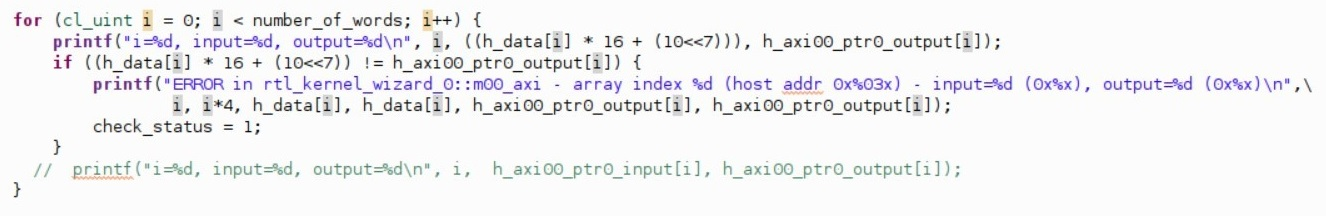
\includegraphics[scale=0.6]{tests_code}}
	\caption{Фрагмент кода функции тестирования}
\end{figure}

Результаты тестов:

\begin{figure}[ph!]
	\center{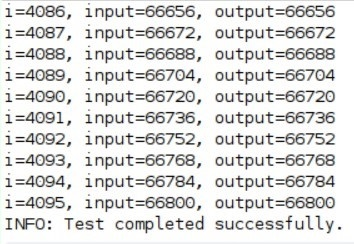
\includegraphics[scale=1.0]{tests}}
	\caption{Результаты тестов}
\end{figure}

\chapter{Вывод}
В ходе лабораторной работы были изучены архитектура гетерогенных вычислительных систем и технологии разработки ускорителей вычислений на базе ПЛИС фирмы Xilinx. Была выполнена генерация ядра ускорителя с последующим синтезом, сборкой и тестированием бинарного модуля ускорителя.
